\documentclass[10pt,letterpaper]{article}
\usepackage[latin1]{inputenc}
\usepackage{amsmath}
\usepackage{amsfonts}
\usepackage{amssymb}
\usepackage{makeidx}
\usepackage{graphicx}
\usepackage{algorithm2e}
\usepackage{float}
\usepackage[left=1.00in, right=1.00in, top=1.00in, bottom=1.00in]{geometry}
\author{Jay Ricco, David Van Chu}
\title{Introduction to Artificial Intelligence\\MNIST and CIFAR10 with Boundary Trees}
\begin{document}
	\maketitle
	\section{Boundary Trees}
		\hspace{5mm}Features are the attributes of an input, or example. With the MNIST data set, each example is composed of 784 pixels, each one of which are considered the features.
		
		\vspace{5mm}
		The Boundary Tree is trained by querying the existing tree using the example as an input, looking for the closest node (using a Euclidean distance as the distance function). When it finds the closest node, if the example is not the same as the closest node, it will add a new node to the tree containing the example.
		
		\vspace{5mm}
		Testing the Boundary Tree involves simply querying the existing tree using an example from the test set. The Boundary Tree determines the class of the example by the class associated with the closest node.

	\section{MNIST}
		\hspace{5mm}Changing the maximum branching factor, k, played a large role in both accuracy as well as the speed of training and querying. As the branching factor grows, it takes longer to train and query, although the accuracy is higher, so it may be worth it depending on the use case.
		For example:
			
		\begin{enumerate}	
			\item with branching factor = $\infty$, averaged over 10 runs
				\begin{itemize}
					\item accuracy = 88$\%$
					\item training = 167.48 seconds
					\item testing = 36.10 seconds
				\end{itemize}
	 		\item with branching factor = 5, averaged over 10 runs
				\begin{itemize}
					\item accuracy = 85$\%$
					\item training = 72.54 seconds
					\item testing = 14.19 seconds
				\end{itemize}
			\end{enumerate}
		
		After running the tests, we noticed that setting the branching factor to 5-10 seemed to be the best if both time and accuracy is a concern, as anything less than 5 will result in lower accuracy while taking about the same amount of time to train and test. With branching factors larger than 10, training and testing time grew quite a bit with only a small increase in accuracy.
		
		Another interesting point is that with a larger branching factor, the training time itself varies by quite a bit, ranging from 140.47 seconds to 223.79 seconds, whereas tests ran with a lower branching factor resulted in consistent training times.
		
		We also tests varying the number of examples we used to train the Boundary Tree. While accuracy and testing time plateaued, the time it took to train grew linearly with more examples.
		
		\begin{figure}[H]
			\caption{MNIST dataset, varying the branching factor, averaged over 10 runs.}
			\centering
			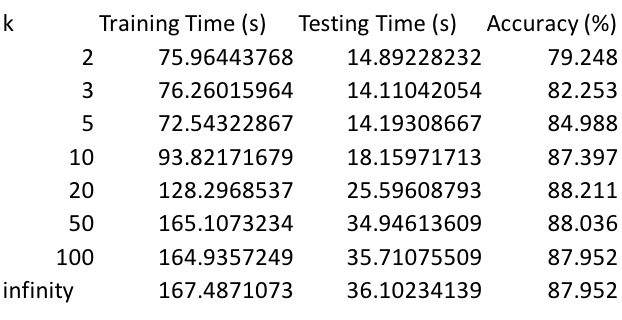
\includegraphics[width=0.60\textwidth]{mnist-varying-k.png}
		\end{figure}
	
	\begin{figure}[H]
		\caption{MNIST dataset, varying the number of examples, averaged over 10 runs.}
		\centering
		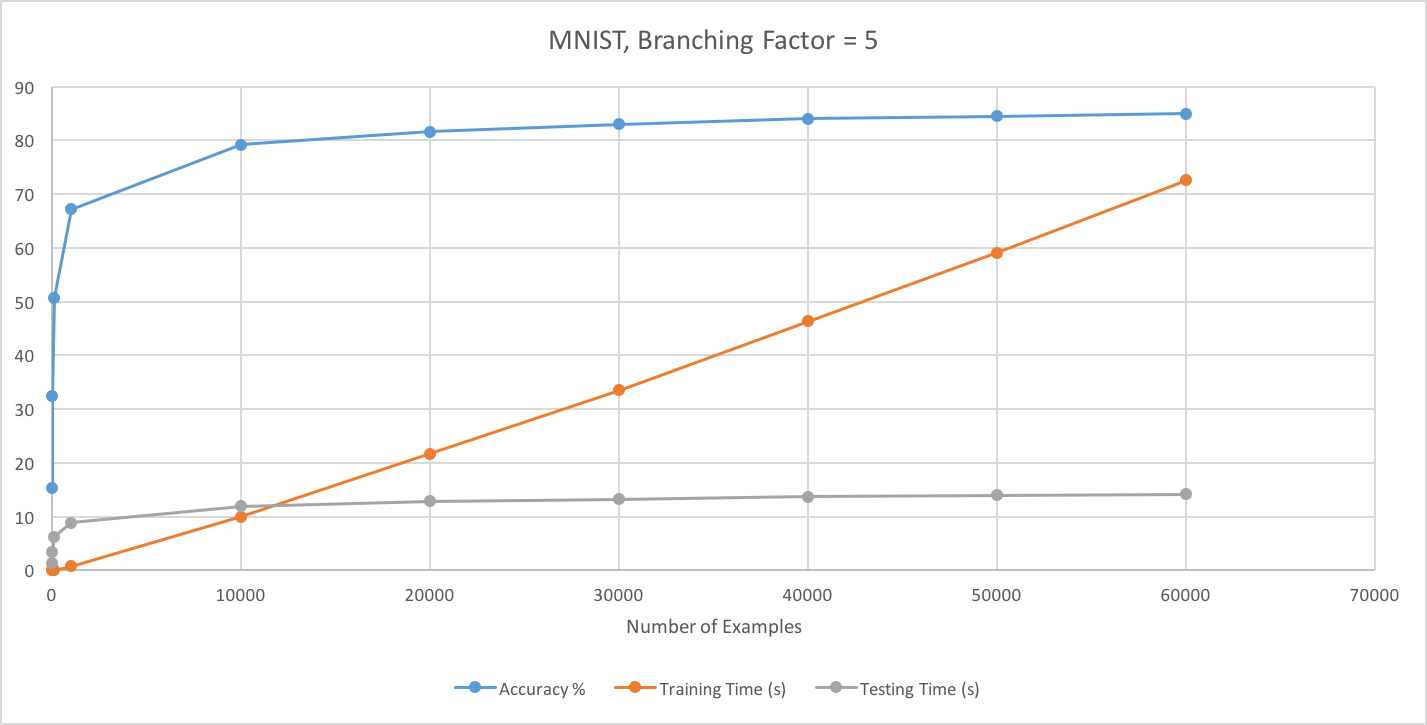
\includegraphics[width=0.60\textwidth]{mnistk5.png}
		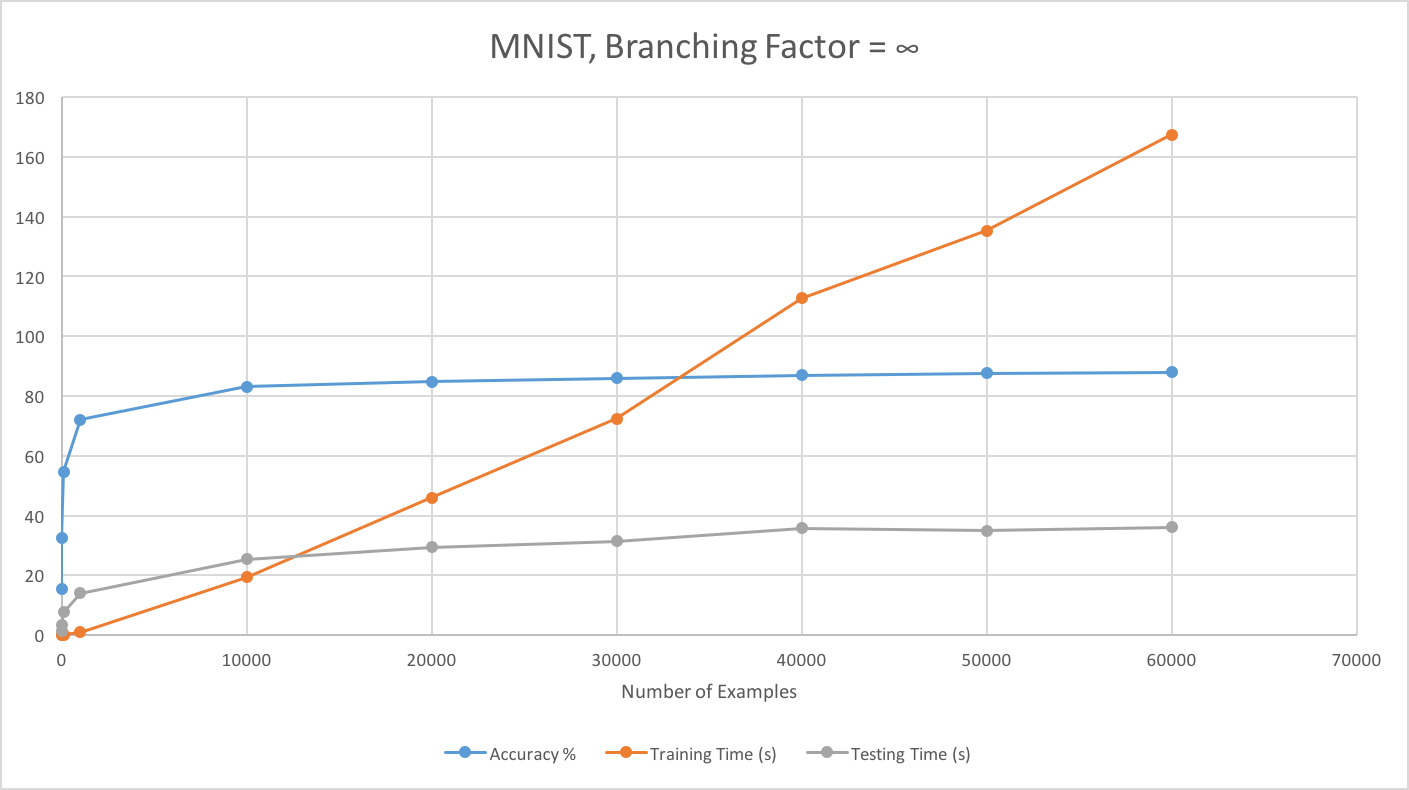
\includegraphics[width=0.60\textwidth]{mnistkinfinity.png}
	\end{figure}
		
		
	\section{CIFAR10}
	\hspace{5mm}We see similar results when using Boundary Trees on the CIFAR10 dataset, although it never achieves over 27.6$\%$ accuracy. Using a smaller branching factor quickens the training time significantly compared to the MNIST dataset results.
	
	\begin{enumerate}	
		\item with branching factor = $\infty$, averaged over 10 runs
		\begin{itemize}
			\item accuracy = 27.3$\%$
			\item training = 125.91 seconds
			\item testing = 52.22 seconds
		\end{itemize}
		\item with branching factor = 5, averaged over 10 runs
		\begin{itemize}
			\item accuracy = 26.5$\%$
			\item training = 32.36 seconds
			\item testing = 10.46 seconds
		\end{itemize}
	\end{enumerate}
	\begin{figure}[H]
	\caption{CIFAR10 dataset, varying the number of examples, averaged over 10 runs.}
	\centering
	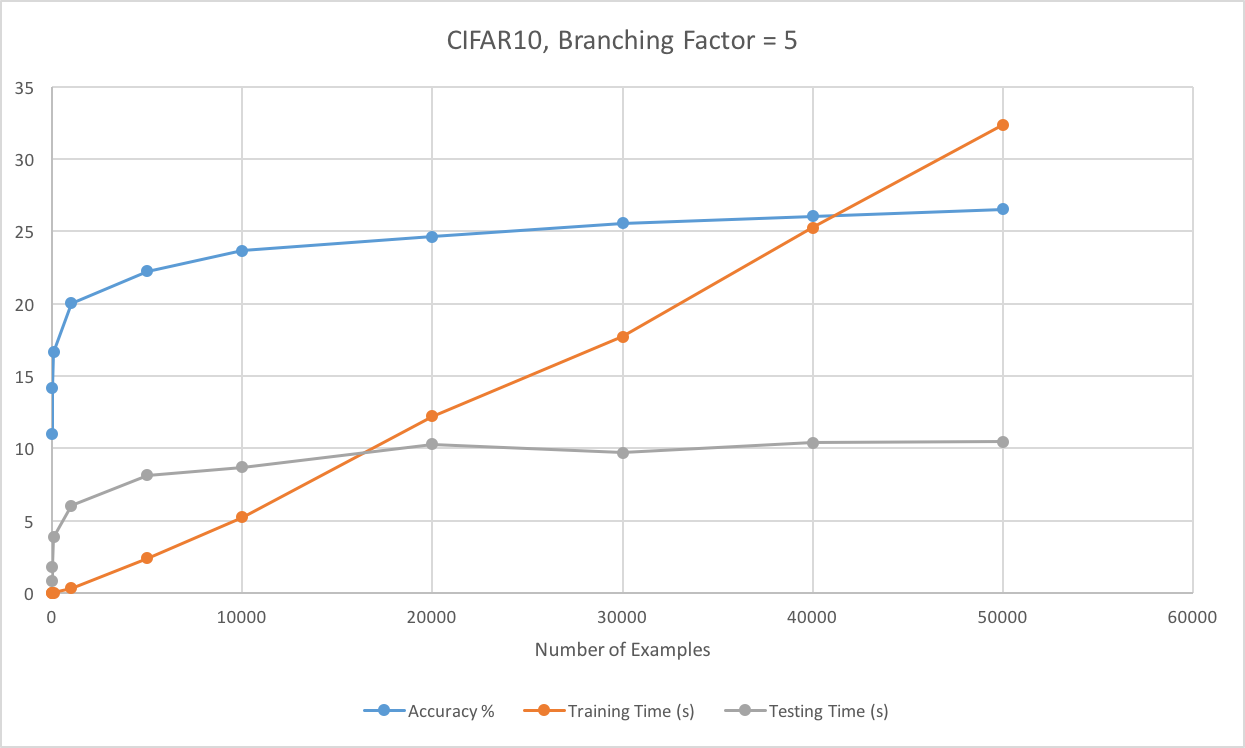
\includegraphics[width=0.60\textwidth]{cifar10k5.png}
	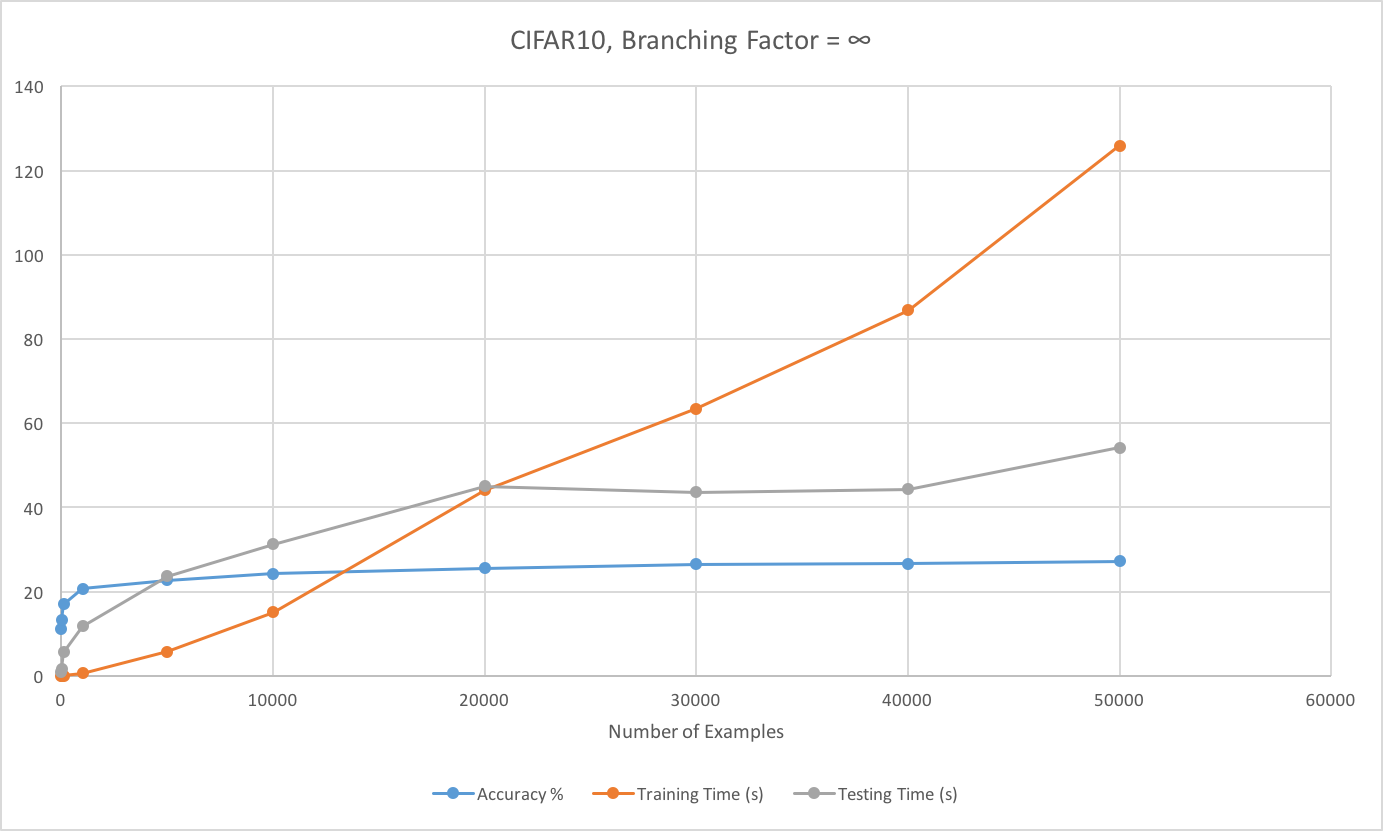
\includegraphics[width=0.60\textwidth]{cifar10kinfinity.png}
	\end{figure}
		
\end{document}